% An alternative to the following \documentclass is
% \documentclass{beamer}
% \mode<presentation>
% {
%   \usetheme{default}
%   \setbeamercovered{transparent}
% }

\documentclass[presentation]{beamer}

% Most of these were autogenerated by org export to beamer.tex file
% I don't know if they are all necessary, but I don't think there is any harm in
% including them. 
\usepackage[utf8]{inputenc}
\usepackage[T1]{fontenc}
\usepackage{graphicx}
\usepackage{grffile}
\usepackage{longtable}
\usepackage{wrapfig}
\usepackage{rotating}
\usepackage[normalem]{ulem}
\usepackage{amsmath}
\usepackage{textcomp}
\usepackage{amssymb}
\usepackage{capt-of}
\usepackage{hyperref}
\usetheme{default}

% I'm not sure what exactly this is for
% It is copied from a template provided by Till Tantau
% <tantau@users.sourceforge.net>
\usepackage[english]{babel}

% It is copied from a template provided by Till Tantau
% <tantau@users.sourceforge.net>
% I'm not sure what exactly this is for
\usepackage{times}

\usepackage{listings}

% Use this to adjust text for overlays
% If set to transparent, then text is overlays is visible, but greyed out.
% If not set, then the text in overlays is not visible at all (i.e., invisible).
\setbeamercovered{transparent}

\usecolortheme{}
\usefonttheme{}
\useinnertheme{}
\useoutertheme{}
\author[Author, Another] % {optional, use only with lots of authors
       {Kit Barton\inst{1} \and \\
        Johannes Doerfert\inst{2} \and \\
        Hal Finkel\inst{2} \and \\
        Michael Kruse\inst{2} \and \\
        Ettore Tiotto \inst{1}}
       
% Give the names in the same order as they appear in the paper.
% Use the \inst{?} command only if the authors have different
% affiliation. 
\institute[IBM Canada and Made up place] % (optional, but mostly needed)
{
  \inst{1}
  IBM Canada
  \inst{2}
  Argonne National Labs
}

% Pick the date.
% Hard code it or pick a floating date based on day the PDF was built.
% Can also be a string
%\date[August 15, 2019]{Name of Conference here}
\date{October 23, 2019}

\title{Writing Loop Optimizations in LLVM}

% Autogenerated by org export to beamer.tex file
\hypersetup{
 pdfauthor={Kit Barton},
 pdftitle={Beamer Template},
 pdfkeywords={},
 pdfsubject={},
 pdfcreator={},
 pdflang={English}}

%\subject{Theoretical Computer Science}
% This is only inserted into the PDF information catalog. Can be left
% out.



% If you have a file called "university-logo-filename.xxx", where xxx
% is a graphic format that can be processed by latex or pdflatex,
% resp., then you can add a logo as follows:

%\pgfdeclareimage[height=0.5cm]{ibm-logo}{/Users/kbarton/Templates/IBMLogo.png}
%\logo{\pgfuseimage{ibm-logo}}

% Delete this, if you do not want the table of contents to pop up at
% the beginning of each subsection:
%% \AtBeginSubsection[]
%% {
%%   \begin{frame}<beamer>{Outline}
%%     \tableofcontents[currentsection,currentsubsection]
%%   \end{frame}
%% }


% If you wish to uncover everything in a step-wise fashion, uncomment
% the following command:

%\beamerdefaultoverlayspecification{<+->}

\begin{document}

% Create the title page
\begin{frame}
  \titlepage
\end{frame}

% Create an outline slide
\begin{frame}{Outline}
  \tableofcontents
  % You might wish to add the option [pausesections]
\end{frame}

% Create a section; comment out if not desired.
\section{Terminology}
\label{sec:terminology}

\begin{frame}[label={sec:org8787e08}]{Loop Representation in LLVM}

  % KB: I will clean this slide up and make it into a proper beamer slide, with
  % animations, if everyone is OK with how it looks.
  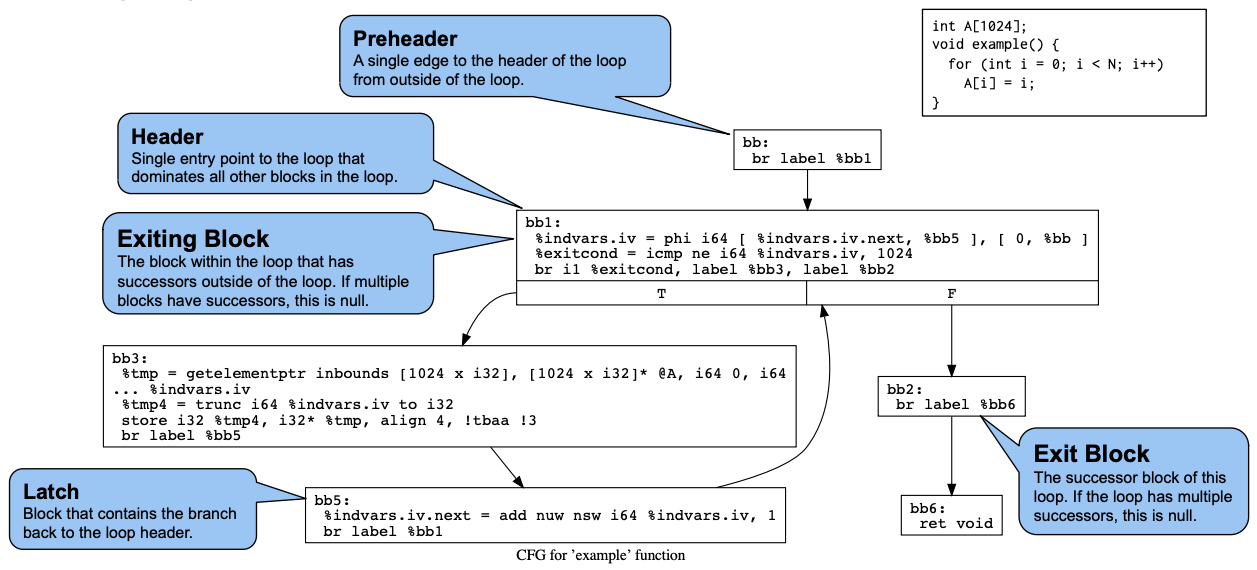
\includegraphics[width=\textwidth]{LoopRepresentation.png}
\end{frame}

\begin{frame}[label={sec:orgac3eb21}]{Other Terminology}
  \begin{block}{}
    \begin{itemize}
    \item Loop predecessor
    \item Backedge taken count
    \item Iteration count
    \item Loop guard 
    \item Others?
    \end{itemize}
  \end{block}
\end{frame}

\begin{frame}[label={sec:rotated}]{Rotated Loops}
  \begin{itemize}
    \item Describe what rotated loops are
    \item Give some examples of rotated loops
    \item Limitations of loop rotation
  \end{itemize}
\end{frame}

\begin{frame}[label={sec:canonical}]{Canonical Form}
Describe loop canonical form - what exactly this entails, \textit{etc}.
\end{frame}

\begin{frame}[label={sec:lcssa}]{Loop Closed SSA Form}
    What exactly is this? When is it useful? What are the implications afterwards?
\end{frame}

\begin{frame}[label={sec:auxdatastruct}]{Auxiliary Data Structures}
    \begin{itemize}
    \item Dominator/PostDominator trees
    \item Data dependence graph (DDG)
    \item Others??
    \end{itemize}
\end{frame}

\section{Considerations when writing a loop pass}
\begin{frame}[label={sec:looppass}]{Loop Pass vs Function Pass}
  \begin{itemize}
  \item What is a loop pass 
  \item What is a function pass 
  \item Differences/pros/cons of using one over the other
  \end{itemize}
\end{frame}

\begin{frame}[label={sec:passmanager}]{Pass Managers}
  \begin{itemize}
    \item New Pass Manager
    \item Legacy Pass Manager
    \item Where to put loop optimizations in the loop opt pipeline (maybe on new slide)
  \end{itemize}
\end{frame}

\section{Other Useful Tools}
\begin{frame}[label=reports]{Reporting success and failure}
  \begin{itemize}
    \item STATISTICS
    \item Optimization Remark Emitter
  \end{itemize}
\end{frame}

\begin{frame}[label={sec:datastructs}]{Updating Data Structures}
    \begin{itemize}
      \item DominatorTreeUpdater
      \item SCEV
      \item Other??
    \end{itemize}
\end{frame}

\end{document}
